\section{Image Crawler}
Classification of real-world images requires a very big dataset for the learning process beforehand. Google Streetview provides 360 degree images from many places in all German urban areas. Using sophisticated crawling techniques, a huge amount of image data can be extracted from these, so called, `Photospheres'.\\
This chapter describes how we used the Google Streetview and other image APIs to crawl images from famous sights in Berlin.

\subsection{Image Crawler}
We provide a Google Streetview image crawling python script inside the\\\texttt{ImageCrawler/streetview_crawler} folder. This script takes a CSV\footnote{Comma-Separated Values} file as input, which specifies the parameters the crawler needs, such as position and viewing angle. Chapter \ref{csv_file} explains the contents of this file.\\
All requirements for the crawler are specified in the \texttt{requirements.txt} file and can be installed with the command \texttt{\$ pip install -r requirements.txt}.\\
Given a location in longitude and latitude, the image crawler will automatically create jpeg-images from different viewing angles. These angles can either be specified or automatically generated by calculating the angle between two geo-coordinates. In the latter case, the script will generate images in five degree steps from 30 degrees to the left to 30 degrees to the right of the calculated viewing angle. If specified by hand, we use one degree steps from the starting to the end angle.\\
Because photospheres can change or get removed, the API uses the closest photosphere to the location provided. This might not be the location specified in the CSV file, which is why we also check the metainformation of each photosphere for the coordinates connected to the image and the status code. In case there is no image in a certain area, the status code tells us that and we don't need to go through all the requests.\\
To prevent Denial-of-Service attacks, the API uses a time- and request-based blocking system. That means, that an IP might be denied further downloads if it either makes request too fast or it reaches the maximum amount. To counter the first blockage, our script uses an exponential wait mechanism. If requests were made too quickly, it waits for a short while before retrying. If it still gets no result, the wait time is increased. This is repeated until the blockage is lifted.\\
For the second part, we provide the usage of a Google API key\footnote{https://developers.google.com/maps/documentation/streetview/}, which can be passed to the crawler script with the \texttt{---key \{key\}} command line switch. The API key enables the crawler to request up to 25'000 requests per day for free, with the option to increase the volume against money.

\subsection{Setup of viewing parameters}\label{csv_file}
Inside the \texttt{places.csv} file, the crawler finds parameters for specified locations and their photospheres.\\
The necessary fields are:
\begin{itemize}
    \item{lat - the latitude of the photosphere in decimal format}
    \item{long - the longitude of the photosphere in decimal format}
    \item{fov - the field-of-view of the photosphere section in degrees}
    \item{pitch - the pitch of the camera in degrees (0 degrees equals parallel to the floor)}
    \item{starthead - the heading from where the camera sweep should start, or 0 if heading should be calculated automatically [optional, if buildingLat and buildingLong specified]}
    \item{endhead - the heading where the camera sweep should end, or 0 if heading should be calculated automatically [optional, if buildingLat and buildingLong specified]}
    \item{name - the name of object in the image; this name is being used as a file prefix for easier identification}
    \item{buildingLat - the latitude of the object in the image; used for automatic heading calculation [optional, if starthead and endhead specified]}
    \item{buildingLong - the longitude of the object in the image; used for automatic heading calculation [optional, if starthead and endhead specified]}
\end{itemize}

The values are read line-by-line and have to be comma-separated.

\subsection{State of Automation}
The static image API we use only provides data about one specific photosphere. This enables us to get a fair amount of images from different viewing angles and different zoom levels for each position specified.\\
As mentioned before, we currently do a camera sweep from a start heading to an end heading, taking one image per degree. This creates on average 40 different viable images. Additionally, we scale each crawled image to 90\% and 80\% of its size, so we gain about 120 images for each line in the CSV file.\\
Unfortunately, this API doesn't provide the possibility to find out which further photospheres are nearby. For example, it is not possible to ``drive down'' a road by pressing the arrows, like on the Google Maps website.\\\\
As a future improvement, the JavaScript API could be used to find out which locations provide images and use this information to crawl more data with less manual work.\\
Also, to improve the quality of the images, it is possible to classify each image with our own sights classifier and find out if the object we search is actually in it and the image is not corrupted by other objects that we might also want to classify.

\subsection{Current Limitations}
Complete automation is not consistently possible at the moment. The static Image API we use for downloading the images does not work on the same database as the JavaScript API, that Google Maps uses. Therefore it is not easily possible to download many of the photospheres from the Streetview web service and results for the same geo-coordinates usually differ between the Image and the JavaScript API. There is currently a feature request open to resolve this issue\footnote{https://code.google.com/p/gmaps-api-issues/issues/detail?id=10402\&q=apitype\%3AStreetView\&sort=-stars\&colspec=ID\%20Type\%20Status\%20Summary\%20Internal\%20Stars}.\\
Another limitation is the reported geo-coordinates in the metadata of the photospheres. These coordinates are usually provided by the camera that took them. GPS can be inaccurate up to 30-40 meters in bad cases. Especially if the image was taken very close to the object, this deviation can cause the automatic calculation of the heading to be wrong and not contain the object observed. This is why the CSV-file also provides the possibility to specify the starting and end heading.

\subsection{Google Places API}
For our project, we use several APIs from Google which help us to get additional information about places. Mainly, this is complementary information such as: Name and address of the place, phone number, website and rating from Google reviews.

\subsubsection{Place Detection API}
The place detection API allows us to discover places close to where the device is located. These are all places registered in Google including local businesses, points of interest, and geographic locations. This API will return a maximum of 10 probable places.
Another very interesting use is that it can help us determinate if our prediction is relevant, by comparing our classification with the results from this function.
\newpage
\subsubsection{How to use it in Android}
The first step is to get an API key from Google\footnote{https://developers.google.com/}. To get the API key, you need to register on the developer console from Google. This platform is used to access every Google API registered by your company.

After that, you need to declare your API key in the android manifest between the \lstinline[language=XML]{<application} tag and the first \lstinline[language=XML]{<Activity>} tag:

\begin{lstlisting}[language=XML, basicstyle=\scriptsize]
<meta-data
android:name="com.google.android.gms.version" android:value="@integer Google_play_services_version"/>
<meta-data
android:name="com.google.android.geo.API_KEY" android:value="API_KEY"/>
\end{lstlisting}

For the third step, you need to ask permissions in the android manifest for Internet access and GPS location.
\begin{lstlisting}[language=XML, basicstyle=\scriptsize]
<uses-permission android:name="android.permission.INTERNET"/>
<uses-permission android:name="android.permission.ACCESS_NETWORK_STATE"/>
<uses-permission android:name="android.permission.ACCESS_FINE_LOCATION"/>
\end{lstlisting}

In your application, you need to declare a "GoogleApiClient" builder and add the APIs you want to use. In our case, and illustrated by the following snippet, we use the \texttt{PLACE\_DETECTION\_API} and \texttt{GEO\_DATA\_API}.

\begin{lstlisting}[language=Java, basicstyle=\scriptsize]
mGoogleApiClient = new GoogleApiClient.Builder(this)
                   .addApi(Places.PLACE_DETECTION_API)
                   .addApi(Places.GEO_DATA_API)
                   .enableAutoManage(this, GOOGLE_API_CLIENT_ID, this)
                   .build()
\end{lstlisting}

The final step is calling the API function. You need to use the \texttt{Places} package associated with the API you want to use. The Google API builder has to be passed to the function.
\begin{lstlisting}[language=Java, basicstyle=\scriptsize]
#For the PLACE DETECTION API
Places.PlaceDetectionApi.getCurrentPlace(mGoogleApiClient, null);

#For the GEO DATA API
Places.GeoDataApi.getPlaceById(mGoogleApiClient, placeId)
\end{lstlisting}

\subsubsection{Limitations}
Google provides a really useful and powerful service, but the requests are very limited. We can only have 1'000 free requests per 24 hours, which is probably not enough enough for a multi-user application.
Therefore, Google provides a business API plan that can be adapted if needed. It gives access to 150'000 request per day and can be increased depending on the number of requests needed.

\subsection{Shutterstock, Flickr and Pinterest}
Shutterstock\footnote{https://www.shutterstock.com/}, Flickr\footnote{https://www.flickr.com/} and Pinterest\footnote{https://www.pinterest.com/} are public web application for hosting and sharing photos and images. For example, on Flickr nearly 7,000 photos are uploaded per minute.
As these services are used by both professional and amateur photographers, we can find a lot of good quality images.

\subsubsection{Example to get images URL}
This is an example about how to get an image URL which can be downloaded, using the angularJS API package and store the resulting image in a mongoDB database.\\
First we create an API object:
\begin{lstlisting}[language=Java, basicstyle=\scriptsize]
var api = shutter.v2({
    clientId: 'Your public key',
    clientSecret: 'Your secret key',
});
\end{lstlisting}

Then we detail the search string we want to crawl. Here we choose the Brandenburg Gate.

\begin{lstlisting}[language=Java, basicstyle=\scriptsize]
var opts = {
    query: 'Brandenburg Gate',
    page: 1,
    per_page: 200,
    sort : 'popular'
};
\end{lstlisting}

Finally, we navigate through the JSON response to get the URL.

\begin{lstlisting}[language=Java, basicstyle=\scriptsize]
    api.image.search(opts, function(err, data) {
        if (err) throw err;

        console.log(data.data[0].id);
        var arrayLength = data.data.length;

        for (var i = 0; i < arrayLength; i++) {
            var obj = data.data[i];
            console.log(obj);
        }
\end{lstlisting}
\newpage
The response return will be as follows.\\
\\
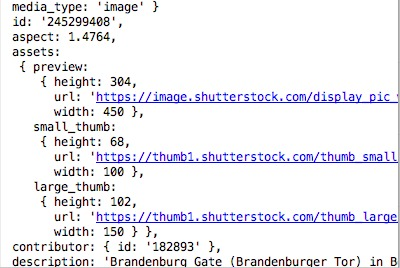
\includegraphics{jsonShutter}

\subsubsection{Limitations}
These services are limited to 3600 call per hours. An API key can be blocked if the service detects an abusive use of the service.
